% !TEX TS-program = pdflatex
% !TEX encoding = UTF-8 Unicode

%%% DOCUMENT DEFINITIONS
% \documentclass[11pt]{article}	% use larger type; default would be 10pt
\documentclass{scrartcl}
\setkomafont{author}{\scshape}
\usepackage{blindtext}
\usepackage[utf8]{inputenc}	% set input encoding (not needed with XeLaTeX)

%%% PAGE DIMENSIONS
\usepackage{geometry}		% to change the page dimensions
\geometry{a4paper}		% or letterpaper (US) or a5paper or....
\geometry{margin=3cm}		% for example, change the margins to 2 inches all round

%%% PACKAGES
\usepackage{wrapfig}
\usepackage{textcomp}
\usepackage{gensymb}
\usepackage{graphicx} 		% support the \includegraphics command and options
\usepackage{booktabs} 		% for much better looking tables
\usepackage{array} 		% for better arrays (eg matrices) in maths
\usepackage{url}
\usepackage{enumitem}
\usepackage{longtable}
\usepackage[defaultlines=4,all]{nowidow}
\usepackage{multicol}

\usepackage{tikz}
\newcommand*\circled[1]{\tikz[baseline=(char.base)]{
        \node[shape=circle,draw,inner sep=2pt] (char) {#1};}}

% Make TOC and URLs clickable
\usepackage[
    colorlinks,
    pdfborder={0 0 0},
    linkcolor=black,
    citecolor=black,
    filecolor=black,
    urlcolor=blue
]{hyperref}

%%% Adjust paragraph indent and spacing
\usepackage{parskip}

%%% HEADERS & FOOTERS
\usepackage{fancyhdr} 		% This should be set AFTER setting up the page geometry
\pagestyle{fancy} 			% options: empty, plain, fancy

%%% More compact item lists
\setlist[itemize]{itemsep=-3pt,topsep=0pt}

%%% TITLE PAGE
\title{
    \vspace*{4cm}
    \huge{zekit} \\
    Instruction and User Guide \\
    \vspace*{0.25cm}
    \small{Revision 1.0 EN - 17/05/2021} \\
    \small{for Firmware V1.00 - 17/05/2021} \\
    \vspace*{0.5cm}
    (Todo: cover image)
    % \includegraphics[scale=0.9]{assets/panel.png}
}
\author{Frédéric Meslin / Fred's Lab}

%%% DOCUMENT
\begin{document}

\maketitle

\pagebreak

% ------------------------------------------------------------------------------------------

%%% TABLE OF CONTENTS
\tableofcontents
\pagebreak

% ------------------------------------------------------------------------------------------

%%% INTRODUCTION
\section{Introduction}

\textbf{Thank you very much for purchasing the zekit!}

The \textbf{zekit} is a 4-voice paraphonic synthesizer kit with digital sound synthesis and an analog filter and VCA. It also features two fully analog envelopes and can be controlled via MIDI and additional clock signals.

You'll learn a lot while building this kit and you'll end up with a cheap and simple but fun instrument that will integrate into your studio setup.

\subsection{Required Skills}

\begin{itemize}
    \item Basic knowledge of analog synthesis
    \item Soldering experience with through-hole (THT) components
    \item Knowledge how to interpret a placement diagram
    \item Knowledge of electronics at an intermediate level
\end{itemize}

\subsection{Required Tools}

In order to fully assemble the kit, you'll need the following tools:

\begin{itemize}
    \item A soldering iron with a tip size around 3mm
    \item Solder with a diameter around 1mm
    \item A wire cutter
    \item A screwdriver
    \item A multimeter (todo: check if required)
\end{itemize}

\subsection{Required Accessories}

\begin{itemize}
    \item Power supply DC 5-9V, 0.5A with barrel connector 5.5mm x 2.5mm, center positive
    \item MIDI cable
    \item Audio cable
    \item Computer or MIDI controller
    \item Audio system
\end{itemize}

% ------------------------------------------------------------------------------------------

\section{Legal notices}

\textbf{Fred's Lab} cannot be liable for erroneous information contained in this manual. The contents of this manual may be updated at any time without prior notice. We have put best effort to ensure the information provided here is useful and accurate. Fred's Lab extends no liabilities in regard to this manual other than those required by the local laws.

\begin{center}
    \textbf{Frédéric Meslin Audiogeräte} \\
    Herwarthstraße, 20 \\
    53115 Bonn, Germany \\
    \url{info@fredslab.net} \\
    \url{http://fredslab.net} \\
\end{center}

\textbf{Support requests} \\
For support requests, you can reach me per e-mail at:
\begin{center}
    \url{support@fredslab.net}
\end{center}
or per post, using the previously mentioned company address.

For each support request, please include the instrument model, serial number and a precise description of the problem encountered with a maximum of details and supporting elements for a quick resolution.

\textbf{Copyright information}

This original manual, its content, including the graphics \& descriptions are the property of \textbf{Fred's Lab}. No part of this manual should be reproduced other than for customer personal use and backup needs without a written permission from \textbf{Fred's Lab}.

\pagebreak

% ------------------------------------------------------------------------------------------

\section{Warranty}
\textbf{Fred's Lab} warranty this product free of defects \textbf{3 years} from its
date of purchase.

This warranty covers product from manufacturing defects, when the product is used observing normal operating conditions. However, the warranty \textbf{does not cover}:

\begin{itemize}
    \item Normal product wear-out
    \item Damages caused by failure to observe the rules of use
    \item Damages due to negligence of the user
    \item Products having been modified or repaired by the user or a third person
\end{itemize}

More information about product warranty can be found in the \textbf{General Terms and Conditions of Sale document} available at:
\begin{center}
    \url{https://fredslab.net/en/terms.html}
\end{center}

% ------------------------------------------------------------------------------------------

\section{Special Thanks}

I would like to thank the following persons for their contributions to this project:

\begin{itemize}
    \item Quality insurance: Benoit Ruelle, René Schmidt, Mathieu Meslin, Oliver Rockstedt
    \item Instruction guide: Oliver Rockstedt
\end{itemize}

% ------------------------------------------------------------------------------------------

\section{Precautions}
Before plugging in the \textbf{zekit!} and go \textbf{rocking the world}, have a sit and read this precautions through:

\begin{itemize}
    \item Always use the device in a dry and warm environment
    \item Never drop the device or expose to too much pressure or vibration
    \item Never spill liquids or bath the device in beer
    \item Never clean the device with an aggressive solvent
    \item Never wiggle the plugs to disconnect the cords
    \item Never connect the line outputs to the power outputs of an amplifier
    \item Only modify the unit at your own risk!
\end{itemize}

\textbf{The zekit} used in conjunction with headphones and speaker systems can produce \textbf{very loud sounds} in a wide range of frequencies.

Human hearing is \textbf{very sensitive} and can be damaged quickly. So watch out your hears and those of your audience!

\pagebreak

% ------------------------------------------------------------------------------------------

\section{Box Content}

\begin{itemize}
    \item PCB with SMD components pre-assembled
    \item 7 tactile switches
    \item 2 toggle switches
    \item 2 potentiometers 10k
    \item 4 potentiometers 100k
    \item 1 power switch
    \item 1 power jack
    \item 1 MIDI jack
    \item 1 audio output jack (6.3mm)
    \item 2 jacks (3.5mm) for clock and input signals
    \item 3 film capacitors
    \item 6 potentiometer knobs
    \item PIC microcontroller IC
    \item Optocoupler IC for VCF/VCA
    \item Optocoupler IC for MIDI
    \item 3 sockets for ICs
    \item Enclosure plates
\end{itemize}

\subsection{The Pre-Assembled PCB}

\subsection{Provided Parts}

(Todo: images with basic descriptions of all parts)

% ------------------------------------------------------------------------------------------

\section{Assembling the Kit}

\subsection{General Advices}

\subsection{Setting Up the Soldering Gig}

\subsection{Soldering the Components}

Order of soldering:

\begin{itemize}
    \item IC sockets
    \item Film capacitors
    \item Trimmers
    \item Tactile switches
    \item Toggle switches
    \item 10k Potentiometers
    \item 100k Potentiometers
    \item Connectors
\end{itemize}

Important remarks:

\begin{itemize}
    \item Polarity of switches
    \item Polarity of sockets (matching the IC direction)
    \item- Taping for easy soldering
    \item Not heat film caps for too long
    \item Solder pots and switches STRAIGHT
          (first solder one leg, press it, then the rest)
\end{itemize}

\subsection{Installing the ICs}

(Todo: maybe power up and measure supply voltages before)

\begin{itemize}
    \item Operational Amplifier
    \item Optocoupler
    \item Microcontroller
\end{itemize}

\section{Power Up and Test}

 (Todo: what to expect)

\subsection{Calibration of the VCF}

(Todo: adjusting the trimmers)

\subsection{Identifying Common Issues}

\begin{itemize}
    \item Bad soldering
    \item Wrong polarity (Todo: of what? ICs?)
\end{itemize}

\pagebreak

% ------------------------------------------------------------------------------------------

\section{Functional Description}

\subsection{Power Supply}

The Zekit needs the energy delivered by the power supply. This block provides 2 voltages: +3.3V and -2V, using a linear regulator and a charge pump respectively.

\subsubsection{Linear Regulator}

\begin{center}
    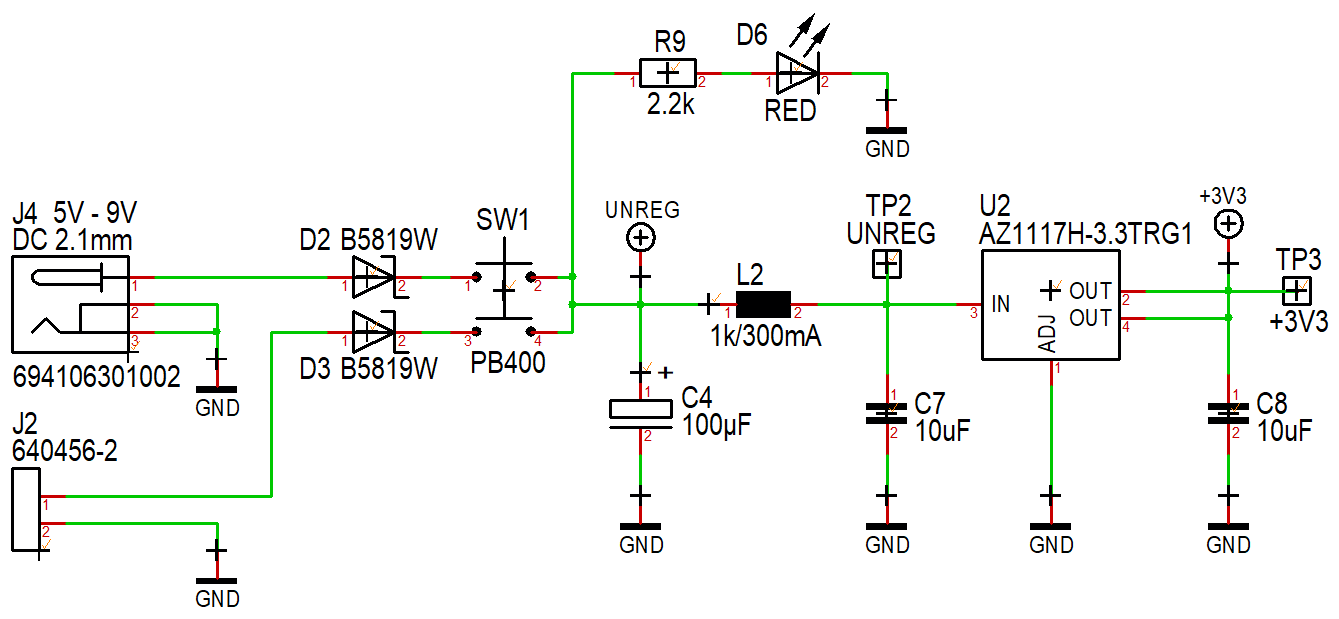
\includegraphics[scale=0.4]{assets/schema-power.png}
\end{center}

\emph{SW1} is the power switch. \emph{D3} ensure voltage polarity is correct, by letting the current flows only in the right direction. \emph{C4}, \emph{R9} \& \emph{C7} filter the input voltage, reducing supply noise. \emph{U2} regulates down the input, assuring a stable +3V3 in all circumstances. \emph{C8} secures \emph{U2} against possible oscillation of its output voltage.

\subsubsection{Charge Pump}

\begin{center}
    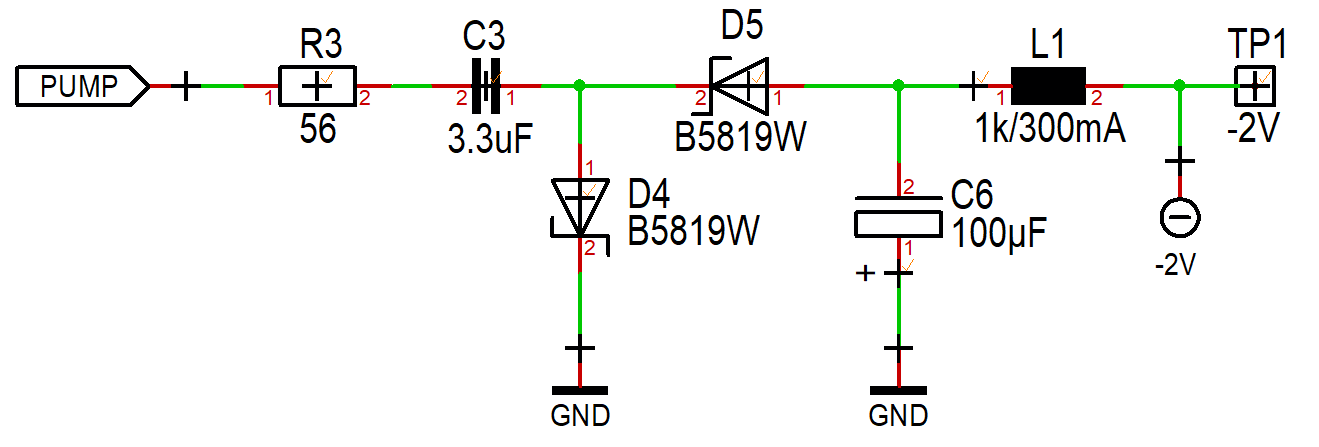
\includegraphics[scale=0.3]{assets/schema-pump.png}
\end{center}

The \emph{PUMP} signal is fed by the microcontroller and alternates between GND and +3.3V at a high frequency. When \emph{PUMP} is at +3.3V, \emph{C3} is charged via \emph{R3} and \emph{D2}, while \emph{D4} is non-conductive. When \emph{PUMP} is at GND, \emph{D2} is isolating and the charge of \emph{C3} is transferred to \emph{C5} via the now conducting \emph{D4}. The inductor \emph{L1} filters the voltage for better noise immunity.

Ideally, the output voltage at \emph{TP1} would be -3.3V, but because of the loss inside the diodes, it will be around -2V, which is still sufficient for proper operation.

\subsection{Microcontroller}

\begin{center}
    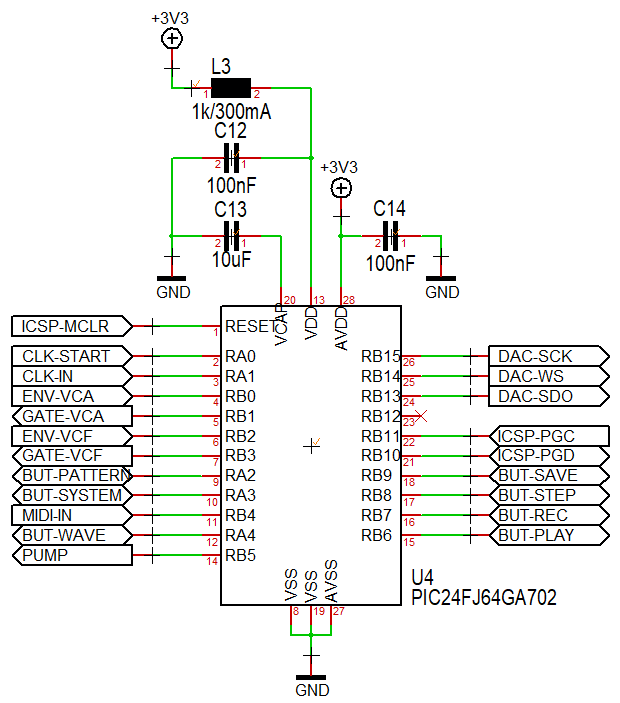
\includegraphics[scale=0.55]{assets/schema-mcu.png}
\end{center}

The microcontroller (MCU) \emph{U7} is the brain of the \textbf{zekit}. It processes all signals from the switches and the inputs and generates the audio waveform as well as some control signals for the analog circuitry. This is done by running a firmware that is stored in the internal flash of the chip. The firmware is pre-programmed by Fred's Lab, but can be replaced by using a dedicated programmer kit.

The capacitors \emph{C11}, \emph{C12} and \emph{C14} are used together with the inductor \emph{L2} to improve the stability of the power supply and reduce noise.

\subsection{DAC}

\begin{center}
    (Todo: DAC schematics)
    % 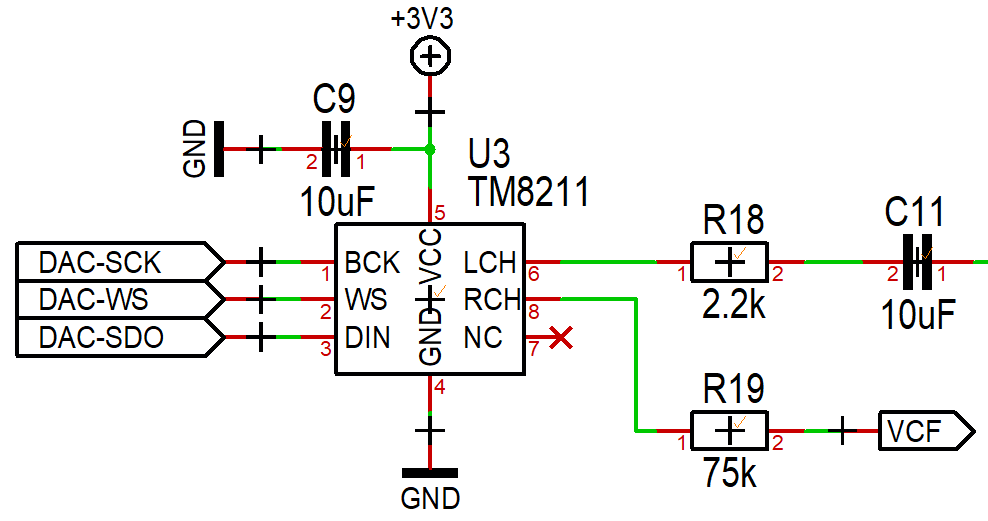
\includegraphics[scale=0.55]{assets/schema-dac.png}
\end{center}

The digital-to-analog converter (DAC) \emph{U3} is directly connected to the microcontroller via 3 signals. It converts the waveform calculated by the MCU into the analog domain. Capacitor \emph{C13} removes the DC offset of the signal, resistor \emph{R19} conditions the level to fit in the range of the next stage (the VCF).

The DAC chip provides two independent output channels of which only one is used internally. The unused channel is routed to the test point \emph{TP4} and can be utilized for additional purposes.

\subsection{Tactile Switches}

\begin{center}
    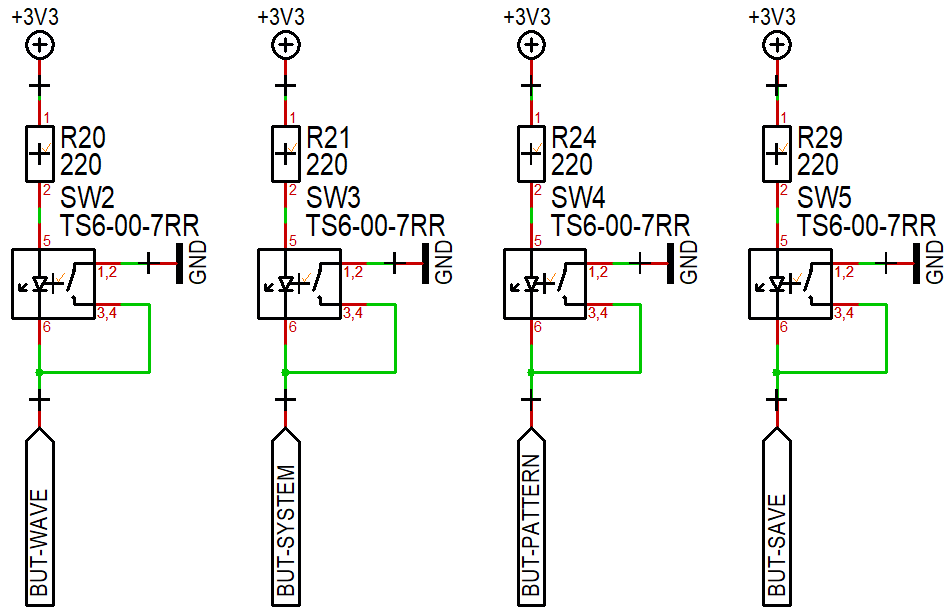
\includegraphics[scale=0.25]{assets/schema-switch.png}
\end{center}

The 7 illuminated tactile switches are directly connected to the microcontroller. The image above shows the \emph{WAVE} button switch \emph{SW2} as an example.

In order to reduce the number of required signal lines, the MCU firmware uses a neat trick: it alternates the mode of the pin connected to the \emph{BUT-WAVE} signal between input and output.

When the MCU pin is configured as input, the button state can be read. In case the button is released, a high level is detected because the pin is connected to +3.3V via the LED and the resistor \emph{R18}. When the button is pressed, the pin is directly connected to GND and a low level is detected. When the MCU pin is configured as output, the LED can be illuminated by driving the signal to GND.

\subsection{VCA}

\begin{center}
    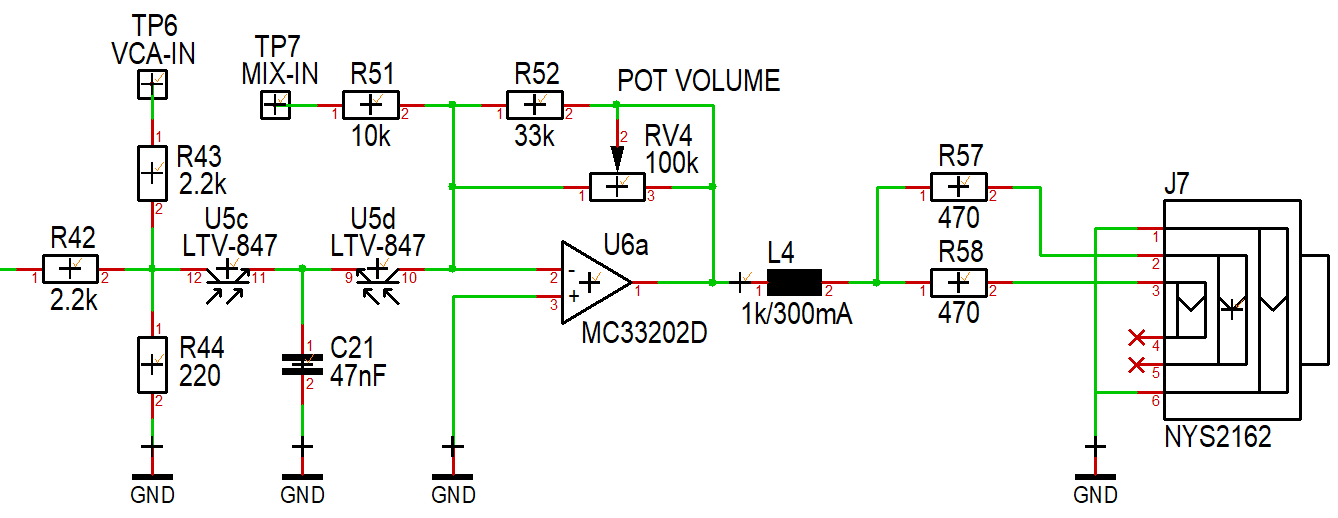
\includegraphics[scale=0.37]{assets/schema-vca.png}
\end{center}

\subsection{VCF}

\begin{center}
    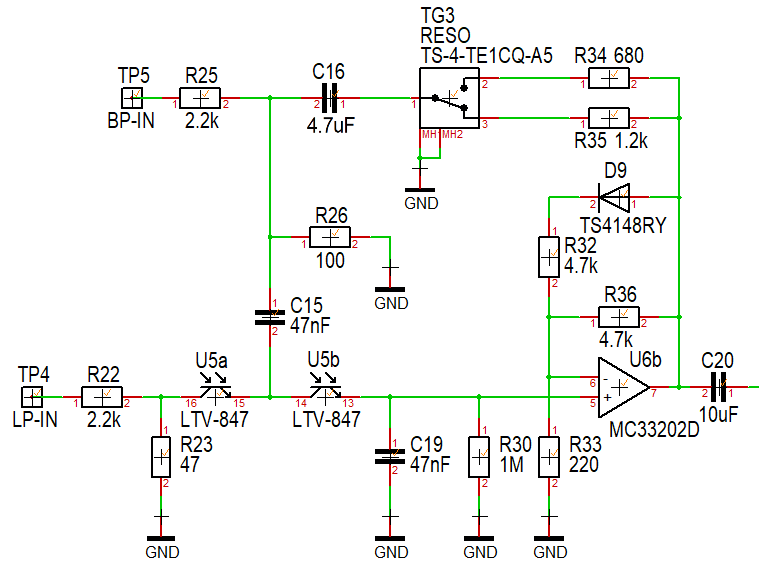
\includegraphics[scale=0.39]{assets/schema-vcf.png}
\end{center}

\subsection{Exponential Control Circuit}

\begin{center}
    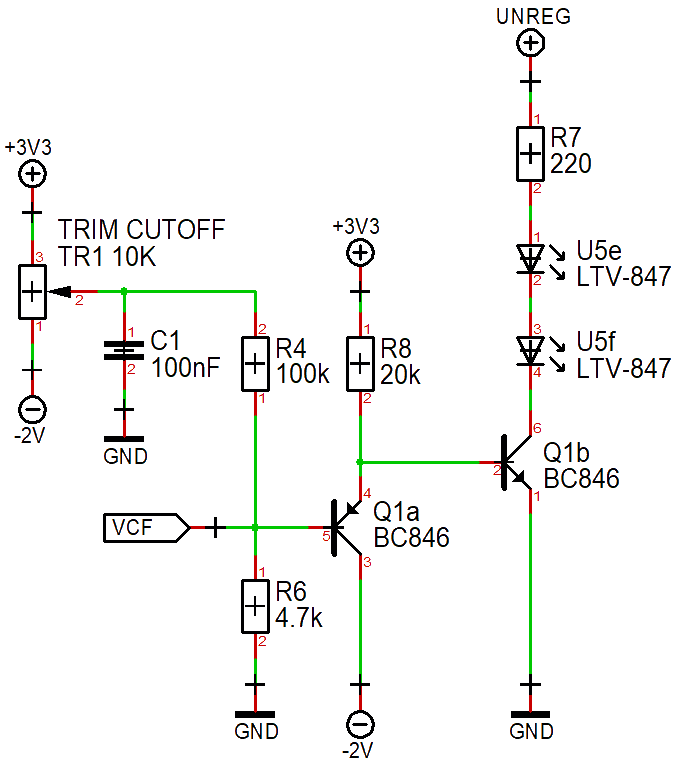
\includegraphics[scale=0.42]{assets/schema-expo.png}
\end{center}

\subsection{Envelopes}

\subsubsection{VCF Envelope}

\begin{center}
    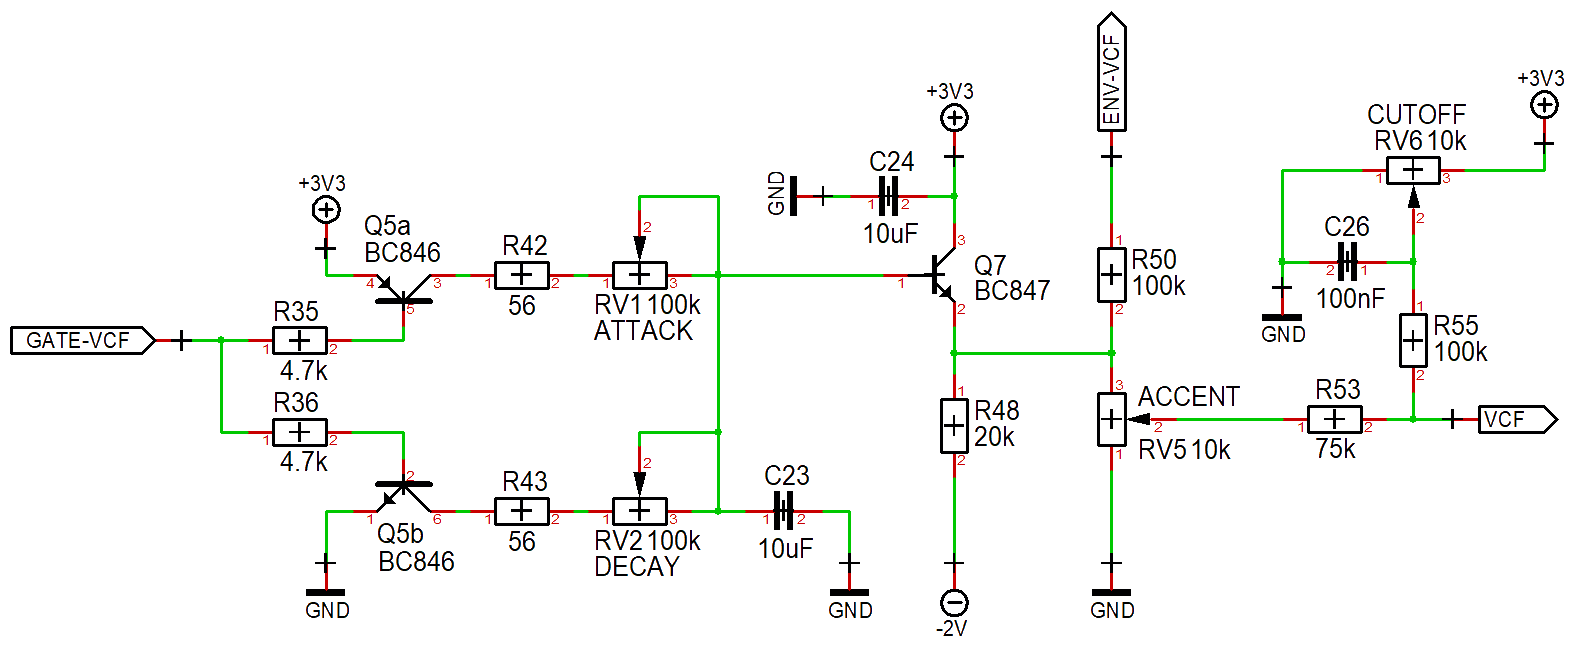
\includegraphics[scale=0.36]{assets/schema-ar.png}
\end{center}

\subsubsection{VCA Envelope}

(Todo: same as VCF envelope but without attack)

\subsection{MIDI Input}

\begin{center}
    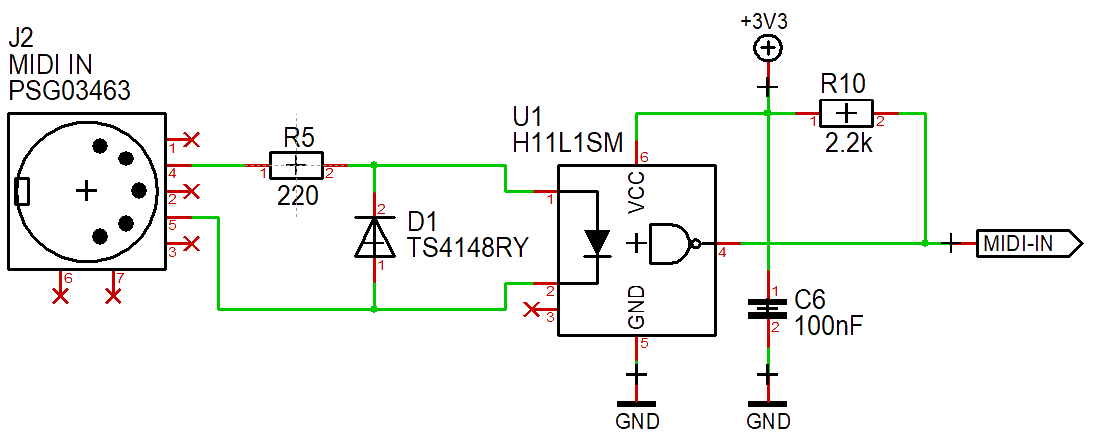
\includegraphics[scale=0.40]{assets/schema-midi.png}
\end{center}

\subsection{Clock Input}

\begin{center}
    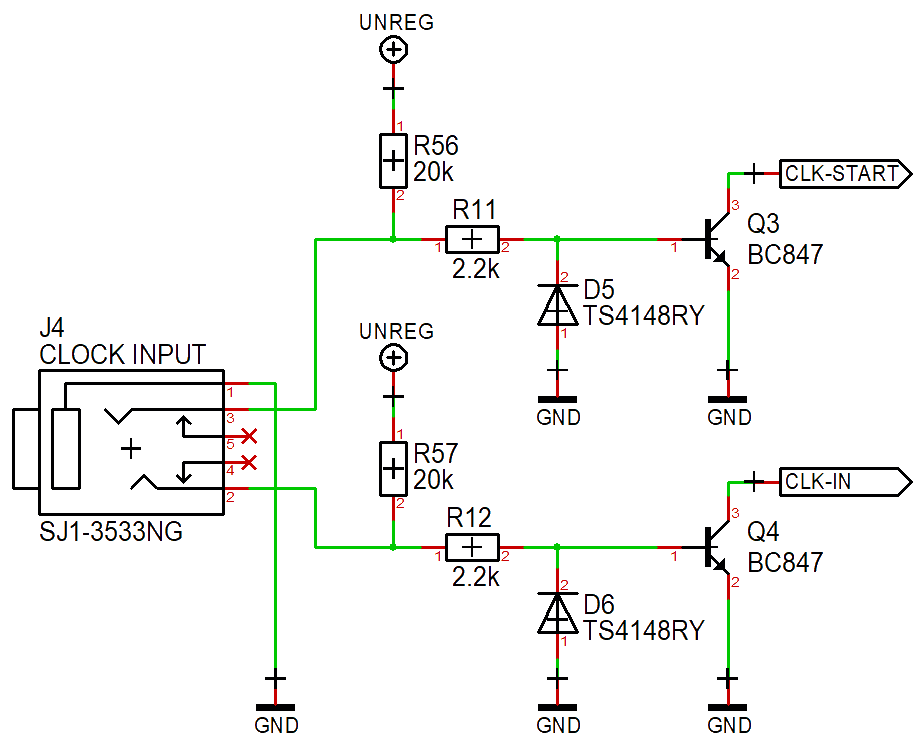
\includegraphics[scale=0.40]{assets/schema-clocks.png}
\end{center}

\pagebreak

% ------------------------------------------------------------------------------------------

\section{Additional Resources}

=> The github
=> The webpage
=> Where to find the MCU source code

\pagebreak

% ------------------------------------------------------------------------------------------

\section{Legal / License}

\pagebreak

% ------------------------------------------------------------------------------------------

\section{Operation}

 (Todo: user manual)

% ------------------------------------------------------------------------------------------

\section{Schematics}

To minimize electronic waste and ensure long product life, Fred’s Lab is willing to provide all technical documents needed to repair his products. The following schematics are provided ”as is” with no warranty of any kind. Any modification made to a Fred’s Lab instrument immediately voids the included 3-year product warranty. Repairs must be carried out by a competent repair service. Fred’s Lab stays available for the maintenance of your instruments. Do not hesitate to contact the support service for a free quote. Spare parts can directly be ordered from us.

\textbf{Intellectual property:}

The following technical documents are provided for advisory, repair and educational purposes only. They remain the entire property of Fred's Lab and cannot be reproduced without a written authorization. Users are granted to draw inspiration from this information for their projects (commercial or not), while respecting the limits of non-cloning or counterfeiting the original product. If in doubt about legal matters, please contact us.

\begin{center}
    (Todo: full schematics)
    % 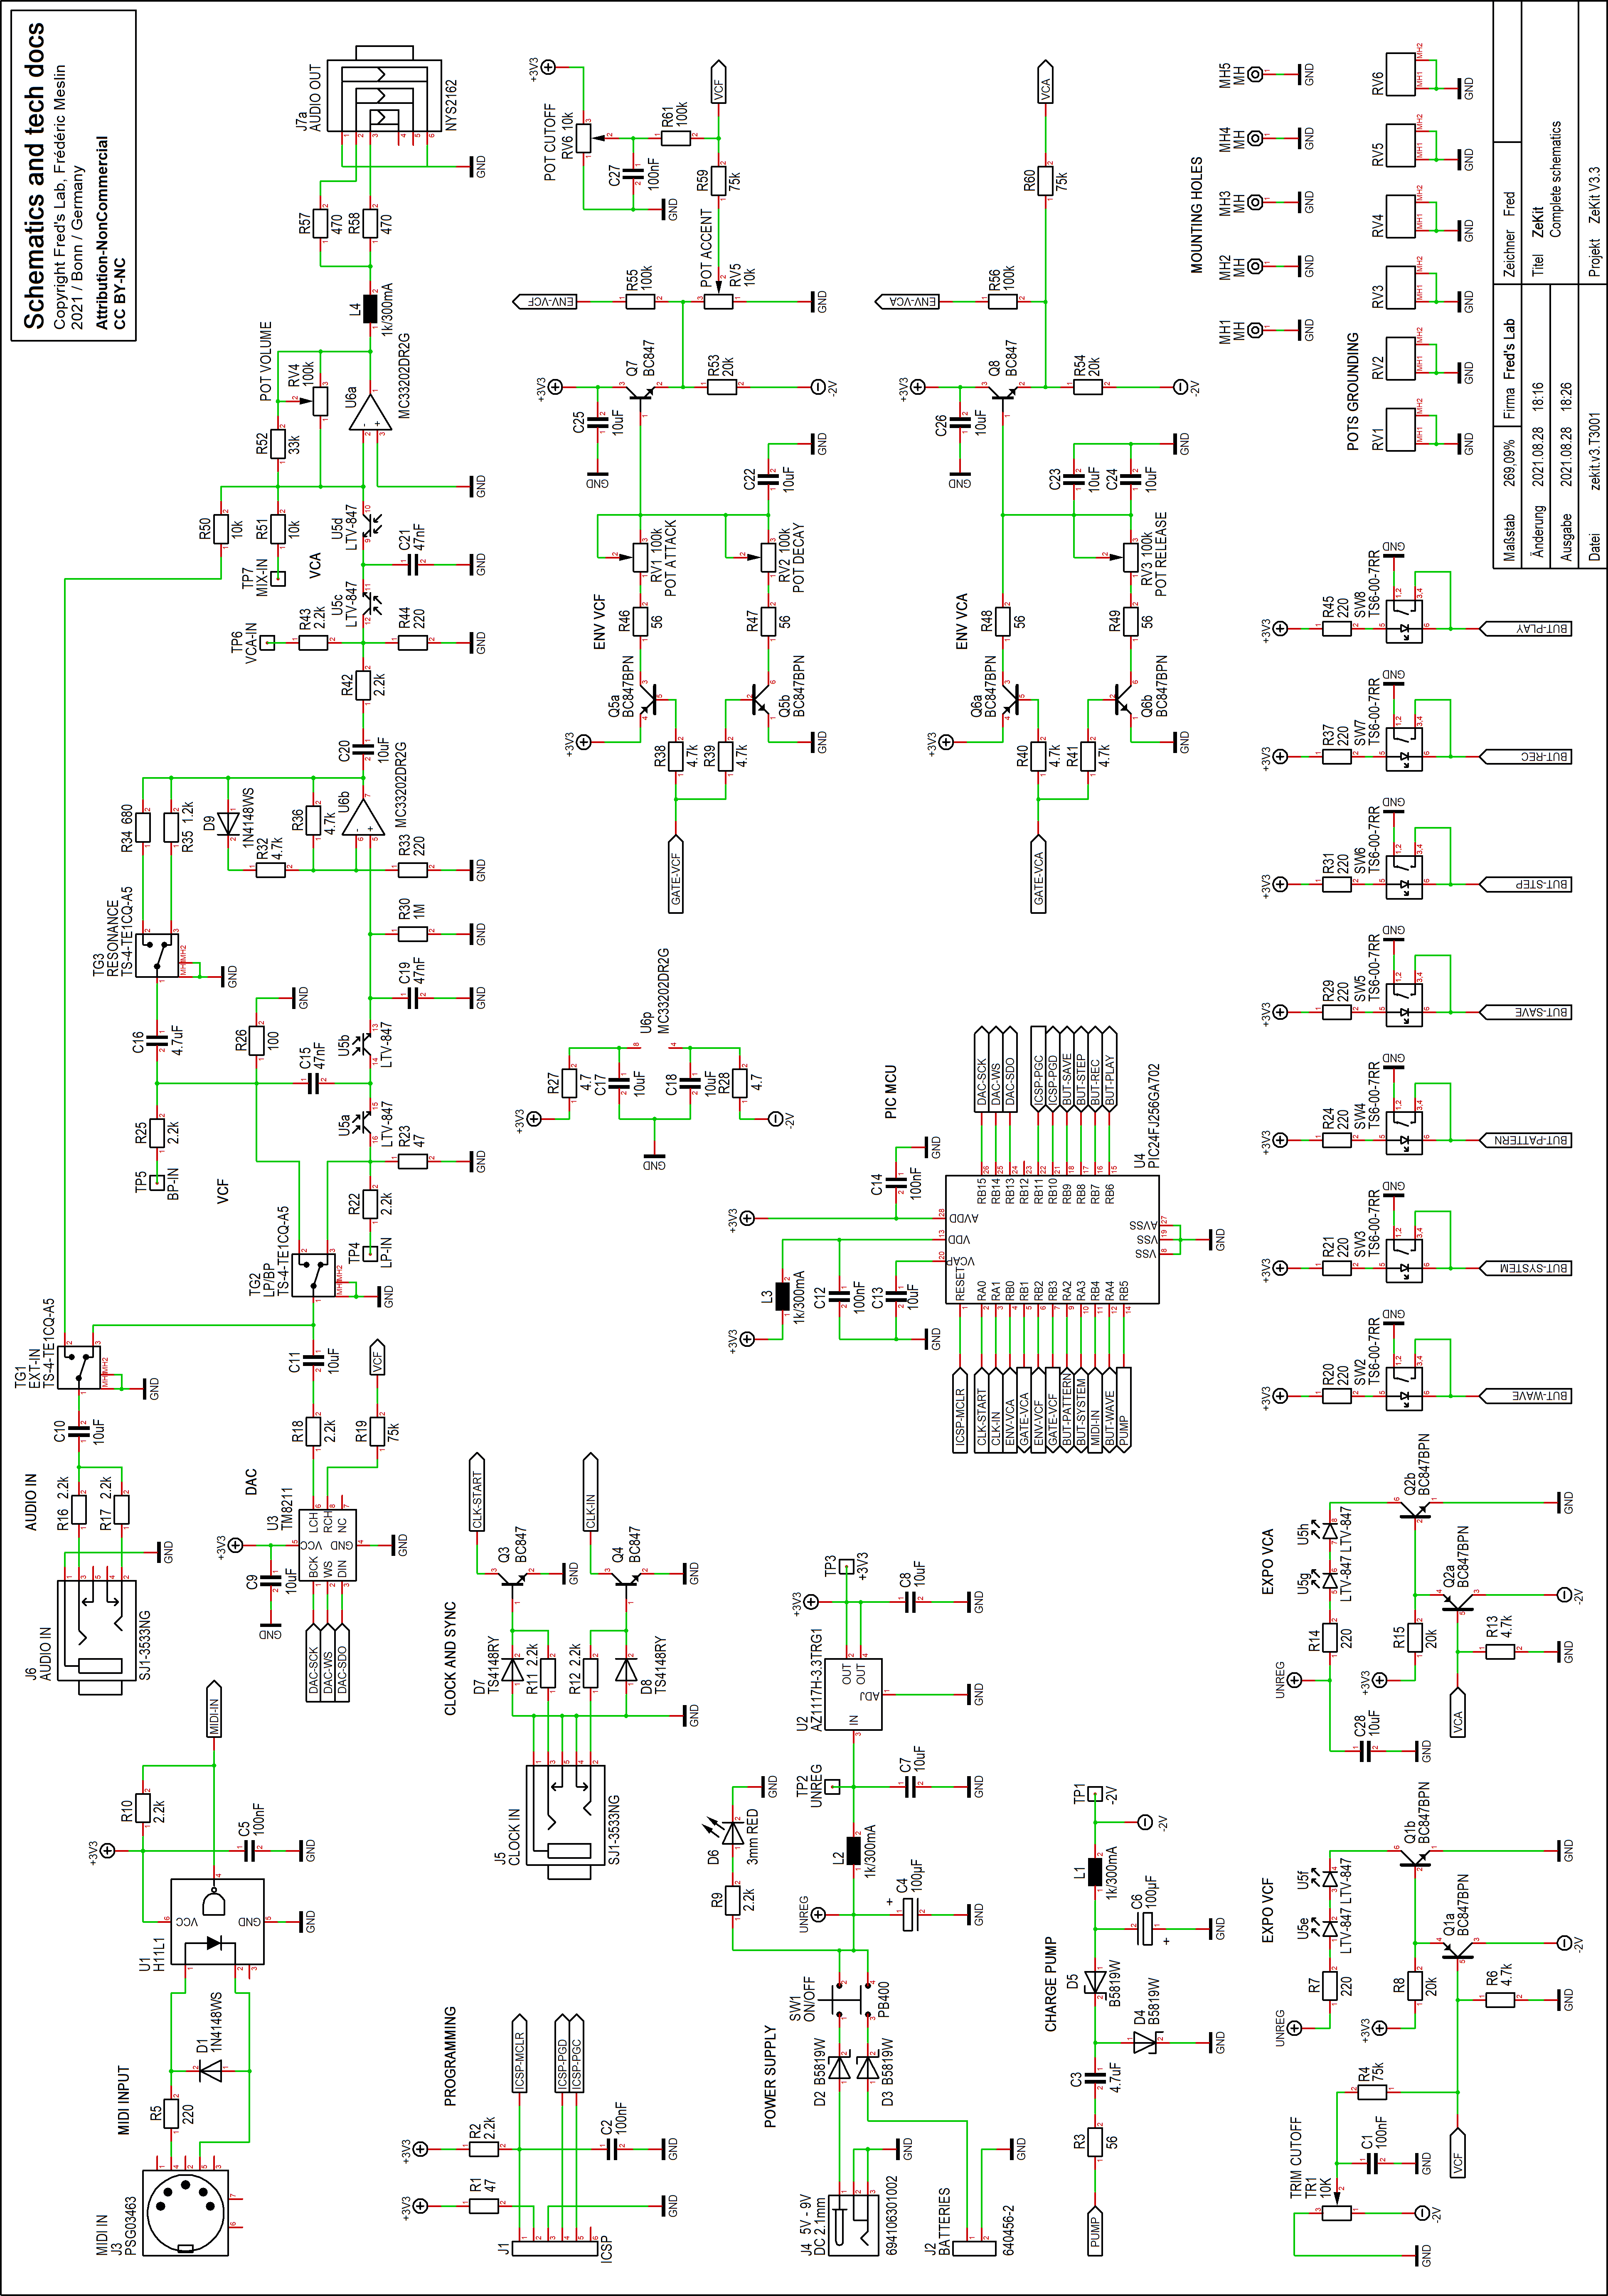
\includegraphics[scale=0.7,angle=90,origin=c]{assets/schema-full.png}
\end{center}
\pagebreak

% ------------------------------------------------------------------------------------------

\section{Norms}
\subsection{Europe: CE}

\begin{center}
    
\includegraphics[scale=0.10]{assets/ce-logo.png}
    \hspace*{1,5cm}
    
\includegraphics[scale=0.05]{assets/weee.png}
\end{center}

\textbf{CE DECLARATION OF CONFORMITY}

1. Product unique identification:

\textbf{zekit} sound module kit \\
\indent Belonging to the category "multimedia electronic equipment"

2. Address of the manufacturer and his authorized representative:

\textbf{Frédéric Meslin Audiogeräte} \\
\indent Herwarthstraße, 20 \\
\indent 53115 Bonn, Germany \\
\indent \underline{Email:} fred@fredslab.net \\
\indent \underline{Telephone:} +49 228 53451657 (office hours)

3. Object of the declaration:

\indent This equipment \textbf{conforms to the following requirements:}

\begin{itemize}
    \item EN 55032:2015 (emission), EN 55035:2017 (immunity)
    \item EN 61000-4-2:2009 (ESD)
    \item EN 61000-4-3:2006 + A1:2008 + A2:2010 (immunity)
    \item EN 61000-4-8:2010 (immunity)
    \item EN 61000-6-3 (interference)
    \item 2011/65/EU (ROHS 2), 2012/19/EU (WEEE)
\end{itemize}

After examinations conducted by the independent laboratory: \\
\indent \textbf{Transferstelle für Elektromagnetische Verträglichkeit} \\
\indent \textbf{Hochschule Koblenz} \\
\indent Konrad-Zuse Straße 1 \\
\indent 56075 Koblenz, Germany \\
\indent \underline{Report:} EMC Testreport (Todo: number/date)

4. Signed for and on behalf of \textbf{Frédéric Meslin Audiogeräte}:

\indent \textbf{Frédéric Meslin}, Lead Engineer of Fred's Lab \\
\indent Bonn, the (Todo: date)

\vspace*{0.25cm}
\indent 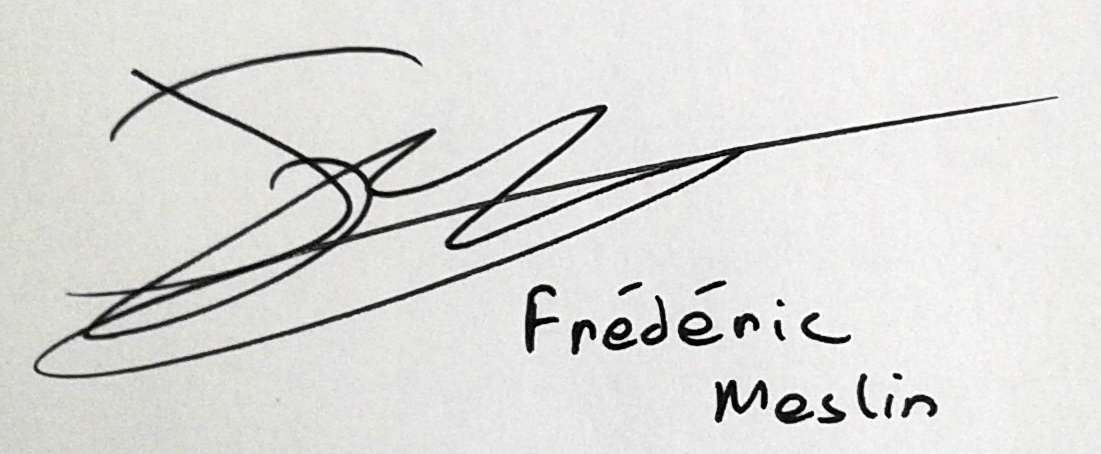
\includegraphics[scale=0.15]{assets/signature.jpg}

\pagebreak

\subsection{Canada: Interference Regulation}
This device does not exceed the Class B limits for radio noise emissions from digital apparatus set out in the radio interference regulation of the Canadian Department of Communications.

Cet équipement n’émet pas de bruits radiofréquence dépassant les limites applicables aux appareils numériques de la Classe B prescrites dans le règlement sur les interférences radio-électriques édicté par le Ministère Des Communications du Canada.

\subsection{USA: FCC Information}

This equipment has been verified to comply with the limits for a class B computing device, pursuant to FCC Rules. In order to maintain compliance with FCC regulations, shielded cables must be used with this equipment. Operation with non-approved equipment or unshielded cables is likely to result in interference to radio and TV reception.

\textbf{Important:} Changes and modifications made to the equipment without the approval of the manufacturer can void your authority to operate this equipment.

\textbf{Note:} This equipment has been tested and found to comply with the limits for a Class B digital device, pursuant to part 15 of the FCC Rules. These limits are designed to provide reasonable protection against harmful interference in a residential installation. This equipment generates, uses and can radiate radio frequency energy and, if not installed and used in accordance with the instructions, may cause harmful interference to radio communications.

However, there is no guarantee that interference will not occur in a particular installation. If this equipment does cause harmful interference to radio or television reception, which can be determined by turning the equipment off and on, the user is encouraged to try to correct the interference by one or more of the following measures:

\begin{itemize}
    \item Reorient or relocate the receiving antenna
    \item Increase the separation between the equipment and receiver
    \item Connect the equipment into an outlet on a circuit different from that to which the receiver is connected
    \item Consult the dealer or an experienced radio/TV technician for help
\end{itemize}


\end{document}
